\section{小波变换}
\subsection{小波变换原理简述}
对非平稳过程,傅里叶变换有其局限性。它只能获取一段信号总体上包含哪些频率的成分,但是对各成分出现的时刻并无所知。因此时域相差很大的两个信号,可能频谱图一样。而加窗截取信号的STFT(短时傅里叶变换)又存在窗长的问题:窗太窄,频率分辨率差;窗太宽,时间分辨率低。于是便产生了利用有限长的会衰减的小波基进行与源信号进行相关的WT(小波变换)和DWT(离散小波变换),需要用到的DWT的变换和逆变换公式如下:
\[
\begin{aligned}
WT[j,k]=\sum_n\langle f,\psi_{j,k}\rangle=\frac{1}{\sqrt{j}}\sum_{n}f[n]\psi[\frac{n-k}{j}]\\
f[n]=\sum_{j,k}\langle f,\psi_{j,k}\rangle\hat{\psi}_{j,k}=\frac{1}{A}\sum_{j,k}WT[j,k]\psi_{j,k}
\end{aligned}
\]

不同于傅里叶变换,变量只有频率$\omega$,小波变换有两个变量:尺度j和平移量 k。尺度j控制小波函数的伸缩,平移量k控制小波函数的平移。尺度j对应于频率(反比),平移量k对应于时间。

\begin{figure}[H]
	\centering
	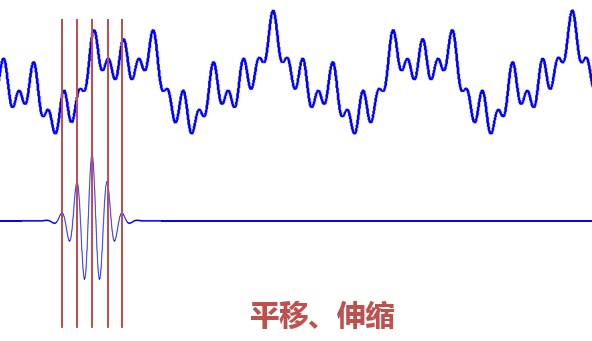
\includegraphics[scale=0.4]{fig2}
	\caption{小波基的尺度参数和平移参数.}
	\label{fig2}
\end{figure}

\subsection{小波变换的滤波器实现与提升算法}
\subsubsection{小波变换的滤波器等效}
小波变换可以用IIR滤波器进行等效(具体推导见《JPEG2000图像压缩基础、标准和实践》),并且可以通过提升算法进行实现。在有损压缩的情况下,JPEG2000标准的核心编码系统默认的不可逆小波变换是Daubechies 9/7 DWT的提升实现,而在无损情况下则采用Le Gall 5/3滤波器的提升实现的整数可逆小波变换。其中Daubechies 9/7是I.Daubechies与M.Antonini等人于1992年提出的一种双正交小波滤波器。Le Gall 5/3是D.Le Gall 与 A.Tabatabai于1988年基于样条5/3变换而提出的一种可逆双正交滤波器。两者的滤波器参数见\textbf{图\ref{fig3}、\ref{fig4}}。其中参数9/7和5/3分别指分解低/高通滤波器的IIR长度,合成滤波器相反(正交对称)。

\begin{figure}[H]
	\centering
	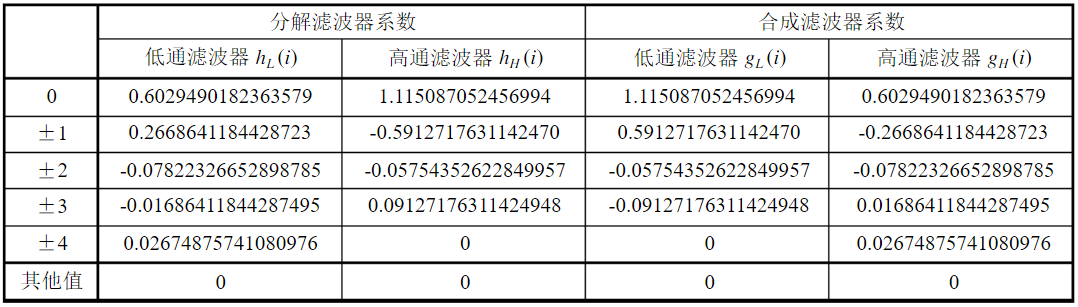
\includegraphics[scale=0.6]{fig3}
	\caption{Daubechies 9/7 滤波器系数表.}
	\label{fig3}
\end{figure}

\begin{figure}[H]
	\centering
	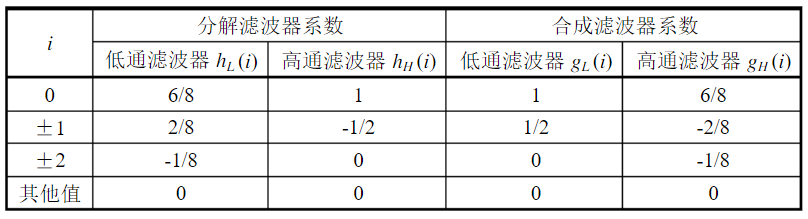
\includegraphics[scale=0.7]{fig4}
	\caption{Le Gall 5/3 滤波器系数表.}
	\label{fig4}
\end{figure}

\subsubsection{小波变换的提升算法}
\paragraph{Daubechies 9/7} 正变换包括4步提升和2步缩放:\par
4步提升:
\[
\begin{aligned}
y(2n+1)&=x(2n+1)-\alpha[x(2n)+x(2n+2)]\\
y(2n)&=x(2n)-\beta[y(2n-1)+y(2n+1)]\\
y(2n+1)&=y(2n+1)+\gamma[y(2n)+y(2n+2)]\\
y(2n)&=y(2n)+\delta[y(2n-1)+y(2n+1)]
\end{aligned}
\]\par
2步缩放:
\[
\begin{aligned}
y(2n+1)&=-Ky(2n+1)\\
y(2n)&=y(2n)/K
\end{aligned}
\]\par

逆变换包括2步缩放和4步提升:\par
2步缩放:
\[
\begin{aligned}
x(2n+1)&=-y(2n+1)/K\\
x(2n)&=Ky(2n)
\end{aligned}
\]\par
4步提升:
\[
\begin{aligned}
x(2n)&=x(2n)-\delta*[x(2n-1)+x(2n+1)]\\
x(2n+1)&=x(2n+1)-\gamma*[x(2n)+x(2n+2)]\\
x(2n)&=x(2n)+\beta*[y=x(2n-1)+x(2n+1)]\\
x(2n+1)&=x(2n+1)+\alpha*[x(2n)+x(2n+2)]
\end{aligned}
\]\par


其中 $\alpha,\beta,\gamma,\delta,K$ 为与滤波器系数有关的参数:$\alpha=1.586134342,\beta=0.052980118,\gamma=0.882911075,\delta=0.443506852,K=1.230174105$。

\paragraph{Le Gall 5/3} 正、逆变换均只需要一步提升与一步缩放。\par
正变换:
\[
\begin{aligned}
y(2n+1)&=x(2n+1)-[x(2n)+x(2n+2)]/2\\
y(2n)&=x(2n)+[y(2n-1)+y(2n+1)+2]/4
\end{aligned}
\]
逆变换:
\[
\begin{aligned}
x(2n)&=y(2n)-[y(2n-1)+y(2n+1)+2]/4\\
x(2n+1)&=y(2n+1)+[x(2n)+x(2n+2)]/2
\end{aligned}
\]

\subsection{二维多级小波变换}
对图像进行2D-DWT后可得到图像的2D-DWT系数,将系数按照左上、左下、右上、右下分别分为LL、LH、HL、HH四个分量(L表示低频,H表示高频)。由于图像的信息大多集中在低频区域,所以若分解所得的LL分量仍含有较多的图像信息时(动态范围大,不利于量化和编码),可将其进一步做2D-DWT分解,也就是多级小波分解,如\textbf{图\ref{fig5}}所示。JPEG2000中一般做$3\sim 4$级2D-DWT,经实践,选用3级2D-DWT就已经足够了。

\begin{figure}[H]
	\centering
	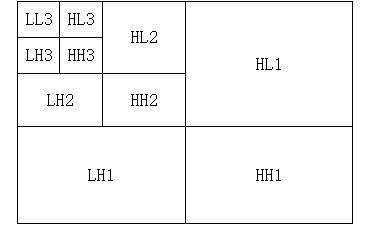
\includegraphics[scale=0.6]{fig5}
	\caption{二维小波变换的多级划分.}
	\label{fig5}
\end{figure}
开始时我用\textit{for}循环实现了提升算法,但是运行速度太慢,于是改为调用\textit{python}的PyWavelets包,建立自定义小波来实现2D-DWT。虽然Daubechies 9/7是以Daubechies命名的,但它和普通的DB族小波基都不同:普通的DB小波基是非对称非正交小波基,而Daubechies 9/7是双正交对称小波基,在查阅官方的小波库文档之后,重新按照双正交对称小波基的参数进行排列,最终实现了基于DB 9/7(有损情况)和LG 5/3滤波器(无损情况)的2D-DWT和2D-iDWT,且速度较原来\textit{for}循环的算法有了很大的提升。\textit{代码见函数dwt和idwt。}


